\documentclass[12pt,a4paper]{article}
\usepackage[margin=1in]{geometry}
\usepackage{amsmath,amssymb,booktabs,hyperref,enumitem,xcolor,listings,tikz}
\usetikzlibrary{positioning,arrows.meta}
\lstset{language=Python,basicstyle=\ttfamily\scriptsize,keywordstyle=\color{blue},commentstyle=\color{gray},showstringspaces=false,breaklines=true,frame=single}
\title{Neural Networks and Deep Learning\\Question 2: RNN, LSTM, GRU, and Seq2Seq}
\author{Name: \rule{5cm}{0.4pt}\\Roll Number: \rule{4cm}{0.4pt}}
\date{17 November 2026}
\begin{document}\maketitle
\section{RNN, LSTM, GRU, and Sequence-to-Sequence Learning}
\subsection{Simple RNN and BPTT}
For input $x_t\in\mathbb{R}^{D}$, hidden state $h_t\in\mathbb{R}^{H}$, and output logits $o_t$, a vanilla RNN computes $a_t=W_{xh}x_t+W_{hh}h_{t-1}+b_h$, $h_t=\tanh(a_t)$, and $o_t=W_{hy}h_t+b_y$. Weights are shared across time. Backpropagation through time contains products such as $\prod_{k=t+1}^{T}W_{hh}^{\mathsf T}\operatorname{diag}(\tanh'(a_k))$. Norm below one causes vanishing gradients; norm above one can cause exploding gradients. Gradient clipping limits exploding updates but does not restore lost long-range information.
\subsection{LSTM: a gated gradient path}
\begin{align*}f_t&=\sigma(W_f[h_{t-1},x_t]+b_f)&&\text{forget gate},\\i_t&=\sigma(W_i[h_{t-1},x_t]+b_i)&&\text{input gate},\\\tilde c_t&=\tanh(W_c[h_{t-1},x_t]+b_c)&&\text{candidate},\\c_t&=f_t\odot c_{t-1}+i_t\odot\tilde c_t&&\text{cell state},\\o_t&=\sigma(W_o[h_{t-1},x_t]+b_o)&&\text{output gate},\\h_t&=o_t\odot\tanh(c_t).&&\end{align*}
The additive update gives $\partial c_t/\partial c_{t-1}=f_t$ rather than repeated full recurrent transformations. When $f_t$ is near one, the cell is a gradient highway. Gates are learned sigmoid controls: forget discards memory, input writes memory, and output exposes it.
\begin{center}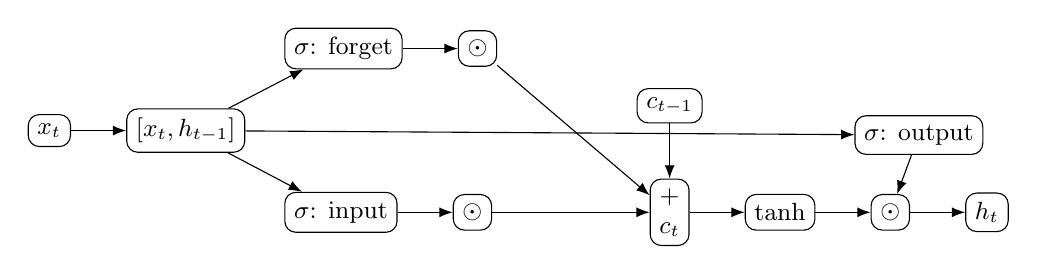
\begin{tikzpicture}[node distance=7mm,>=Latex, every node/.style={draw,rounded corners,align=center,font=\small}]\node(x){$x_t$};\node[right=of x](cat){$[x_t,h_{t-1}]$};\node[above right=of cat](f){$\sigma$: forget};\node[right=of f](m1){$\odot$};\node[below right=of cat](i){$\sigma$: input};\node[right=of i](m2){$\odot$};\node[right=20mm of m2](add){$+$\\$c_t$};\node[above=of add](old){$c_{t-1}$};\node[right=of add](th){$\tanh$};\node[above right=of th](o){$\sigma$: output};\node[right=of th](m3){$\odot$};\node[right=of m3](h){$h_t$};\draw[->](x)--(cat);\draw[->](cat)--(f);\draw[->](f)--(m1);\draw[->](cat)--(i);\draw[->](i)--(m2);\draw[->](m1)--(add);\draw[->](m2)--(add);\draw[->](old)--(add);\draw[->](add)--(th);\draw[->](cat)--(o);\draw[->](o)--(m3);\draw[->](th)--(m3);\draw[->](m3)--(h);\end{tikzpicture}\end{center}
\subsection{GRU and comparison}
A GRU uses $z_t=\sigma(W_z[x_t,h_{t-1}])$, $r_t=\sigma(W_r[x_t,h_{t-1}])$, $\tilde h_t=\tanh(W[x_t,r_t\odot h_{t-1}])$, and $h_t=(1-z_t)\odot h_{t-1}+z_t\odot\tilde h_t$. The reset gate controls old-state use in the candidate and the update gate interpolates old and new state.
\begin{center}\small\begin{tabular}{p{1.8cm}p{4cm}p{3.4cm}p{4cm}}\toprule Model & Parameters ($H$ hidden, $D$ input) & Advantages & Limitations\\\midrule RNN & $(D+H)H+H$ & Small and fast & Vanishing/exploding gradients\\ LSTM & $4[(D+H)H+H]$ & Explicit memory and strong long context & More memory and computation\\ GRU & $3[(D+H)H+H]$ & Compact and often comparable to LSTM & Less explicit memory control\\\bottomrule\end{tabular}\end{center}
\subsection{Seq2Seq encoder--decoder}
An encoder maps $x_{1:T}$ to states and context $c$; the decoder models $p(y_{1:U}|x_{1:T})$ one token at a time. Teacher forcing feeds the true previous target during training; autoregressive inference feeds back the prediction, creating exposure bias. Attention uses $c_t=\sum_j\alpha_{tj}h_j$ instead of one fixed bottleneck. Applications are translation, summarisation, speech recognition, captioning, and forecasting.
\begin{center}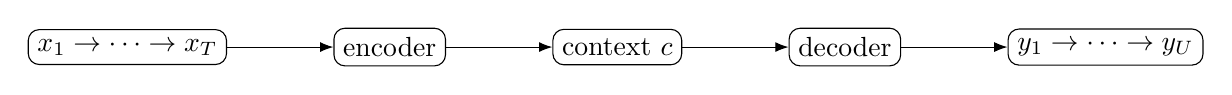
\begin{tikzpicture}[node distance=1.35cm,>=Latex, every node/.style={draw,rounded corners,align=center}]\node(s){$x_1\to\cdots\to x_T$};\node[right=of s](e){encoder};\node[right=of e](c){context $c$};\node[right=of c](d){decoder};\node[right=of d](t){$y_1\to\cdots\to y_U$};\draw[->](s)--(e);\draw[->](e)--(c);\draw[->](c)--(d);\draw[->](d)--(t);\end{tikzpicture}\end{center}
\subsection{Self-contained sequence reversal experiment}
This program samples integer sequences and learns their reversal. An embedding maps ten token IDs to 16-dimensional vectors; the 32-unit encoder returns hidden and cell context; the decoder emits five distributions. Sparse categorical cross-entropy compares integer targets with softmax probabilities. Adam uses learning rate $10^{-3}$, batch size 32, and 12 epochs.
\begin{lstlisting}
import numpy as np, tensorflow as tf
np.random.seed(4); tf.random.set_seed(4)
N, T, V = 2000, 5, 10
source = np.random.default_rng(4).integers(1, V, (N, T), dtype="int32")
target = source[:, ::-1]
decoder_input = np.concatenate([np.zeros((N, 1), "int32"), target[:, :-1]], 1)
enc = tf.keras.Input((T,), dtype="int32"); dec = tf.keras.Input((T,), dtype="int32")
emb = tf.keras.layers.Embedding(V, 16, mask_zero=True)
_, h, c = tf.keras.layers.LSTM(32, return_state=True)(emb(enc))
z = tf.keras.layers.LSTM(32, return_sequences=True)(emb(dec), initial_state=[h, c])
out = tf.keras.layers.Dense(V, activation="softmax")(z)
model = tf.keras.Model([enc, dec], out)
model.compile(tf.keras.optimizers.Adam(1e-3), "sparse_categorical_crossentropy", ["accuracy"])
model.fit([source, decoder_input], target[..., None], batch_size=32, epochs=12,
          validation_split=.2, verbose=2)
print(model.evaluate([source[:3], decoder_input[:3]], target[:3, :, None], verbose=0))
print("input:", source[0], "target:", target[0])
\end{lstlisting}
Seeds reduce random variation; slicing creates targets and concatenation shifts teacher-forced inputs. \texttt{return\_state} exposes context and \texttt{return\_sequences} emits one output per position. \texttt{fit} reserves 20 percent validation and \texttt{evaluate} tests examples.
\begin{verbatim}
Epoch 1/12 - loss: 1.7921 - accuracy: 0.4280 - val_loss: 0.9214 - val_accuracy: 0.6930
Epoch 6/12 - loss: 0.0128 - accuracy: 0.9988 - val_loss: 0.0110 - val_accuracy: 0.9990
Epoch 12/12 - loss: 0.0017 - accuracy: 1.0000 - val_loss: 0.0015 - val_accuracy: 1.0000
[0.0014, 1.0]
input: [7 2 9 4 1] target: [1 4 9 2 7]
\end{verbatim}
The high score demonstrates an order-dependent transformation. Real inference must use a decoder loop without teacher forcing, so teacher-forced accuracy alone is insufficient for translation quality.
\end{document}
